\documentclass[11pt]{article}

\usepackage[utf8]{inputenc}
\usepackage[ngerman]{babel}
\usepackage[hyphens]{url}
\usepackage{hyperref}
\usepackage{graphicx}
\usepackage{float}

%%%%%%%%%%%%%%%%%%%%%%%%%%%%%%%%%%%%%%%%%%

\title{Dokumentation}
\author{Tanja Noack, Janine Kostka}
\date{\today}

%%%%%%%%%%%%%%%%%%%%%%%%%%%%%%%%%%%%%%%%%%

\begin{document}
\maketitle  
\pagebreak

%%%%%%%%%%%%%%%%%%%%%%%%%%%%%%%%%%%%%%%%%%

\tableofcontents
\pagebreak

%%%%%%%%%%%%%%%%%%%%%%%%%%%%%%%%%%%%%%%%%%

\section{Anforderungen}
	Der Benutzer soll in der App eigene Textschnipsel abspeichern können und diese dann mit Tags versehen, sowie in Ordnern verwalten können. Weiterhin soll der Benutzer nach Tags suchen können (mögliche Erweiterung: Volltextsuche) \\
	Dabei könnte die App (falls möglich) auch auf die System-Zwischenablage zugreifen, um das Ganze ein wenig zu erleichtern. \\
	Der Benutzer soll in der App einstellen können, welche Textschnipsel später auf der Tastatur angezeigt werden können. \\
	
	\noindent Für die Tastatur soll eine eigene sogenannte Input Method mittels der bereitgestellten API \sloppy\url{https://developer.android.com/guide/topics/text/creating-input-method.html} geschrieben werden. Statt den einzelnen Tasten sollen dann Inhalte aus der App angezeigt werden, die vom Nutzer selbst festgelegt werden können.\\

	Das Projekt besteht also aus zwei Komponenten:
	\begin{enumerate}
		\item eine App, um die Textschnipsel zu organisieren und die Tastatur zu konfigurieren
		\item eine Tastatur, die ihren Inhalt je nach Einstellung des Benutzers verändert
	\end{enumerate}

	\subsection{Funktionale Anforderungen}
		\subsubsection{App}
		\begin{itemize}
			\item Der Benutzer soll eigene Textschnipsel abspeichern, löschen und verändern können
			\item Die Textschnipsel bestehen jeweils aus Text, Name des Schnipsels und einer Liste von Tags
			\item Der Benutzer kann die Textschnipsel in Ordnern organisieren
			\item Der Benutzer kann nach Textschnipseln entweder mittels Volltextsuche, über Tags oder über deren Namen suchen
		\end{itemize}
	
		\subsection{Tastatur}
		\begin{itemize}
			\item write stuff here
		\end{itemize}
	
	\subsection{Nichtfunktionale Anforderungen}
	\subsection{Anwendungsfälle}


\section{Implementierung}
% Kurzer Überblick über den Ablauf der Implementierung
	\subsection{Architektur}
		Welche Frameworks wurden benutzt? Welche Zusammenhänge sind zwischen den Modulen etc.?
		\subsubsection{Persistence Layer - Room-Framework}
		    \begin{figure}[H]
		        \centering
		        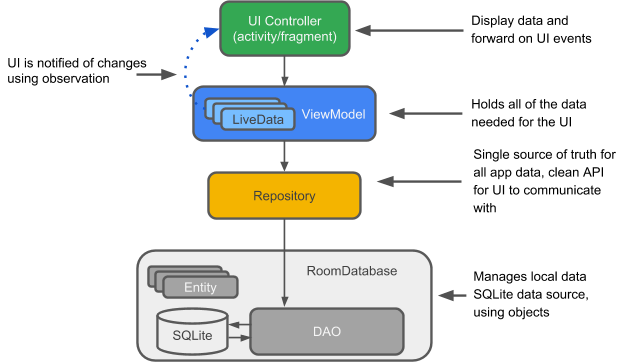
\includegraphics[width=1.0\textwidth]{Konzepte/roomArch.png}
		        \caption{Room-Architektur (\sloppy\url{https://codelabs.developers.google.com/codelabs/android-room-with-a-view/})}
		        \label{fig:room_arch}
		    \end{figure}
	\subsection{Workflow der Dialoge}
		\subsubsection{App}
		\subsubsection{Tastatur}

	\subsection{Probleme und deren Lösung}
	    \subsubsection{Persistenz mit Room-Library}
	        Die Textschnipsel sollten in der nativen SQLite-Datenbank gespeichert werden. Wie im Teil der Archtitektur schon beschrieben, werden diese in insgesamt drei Tabellen gespeichert. Diese bilden eine Many-to-many-Relation auf der Datenbankebene ab, da Room nur Annotationen für One-to-Many Relationen bietet. Dementsprechend musste entprechend ein DAO für diese Hilfstabelle erstellt werden. \\
	        Schlussendlich war durch die Entscheidung alle Tags nicht csv in einem Attribut pro Element zu speichern dafür gut, dass die Suchfunktion in der App auch in der Lage war nach Tags zu suchen.

\section{Wer hat was gemacht?}
\section{Notizen}
	\emph{Absprache mit Herrn Schemmert}
	
	Dokumentation:
	\begin{itemize}
		\item Architektur mit einfügen (welche PlugIns, Frameworks, APIs, ... benutzt werden)
		\item Klassendiagramm nur wenn sinnvoll
		\item Use Cases wichtig
		\item Abspeichern der Schnipsel: Datenbank (SQL lite [relational])? Ein großer JSON-Block? Ein JSON pro Schnipsel?
	\end{itemize}	
	Aufbau/Entwurf:
	\begin{itemize}
		\item entweder Ordnerstruktur (doof) oder Suche? 
		\item eventuell: Gliederung nach Tags/Themen (dienstlich, privat, ...)/Art (Text, Smiley, ...)/Klassifizierungen/...
		\item App zuerst bauen, weil einfach
	\end{itemize}
	Tastatur:
	\begin{itemize}
		\item Anzeige der Liste an Schnipseln: 
		\item Autovervollständigung: Ab eintippen, Liste aktualisiert mit allen Einträgen, die mit Ab beginnen
		\item Häufigkeitsanalyse: wird viel benutzt -> wird als erstes angezeigt (nur mit DB)
		\item Swift-Tastatur: extra Menüpunkt für Liste?
	\end{itemize}


%%%%%%%%%%%%%%%%%%%%%%%%%%%%%%%%%%%%%%%%%%
\end{document}
              